% -*- root: ../main.tex -*-
%!TEX root = ../main.tex
% this file is called up by main.tex
% content in this file will be fed into the main document
% vim:textwidth=80 fo=cqt

\chapter{Introduction}\label{ch:intro}
\section{Chemistry}\label{subsec:liionchemistry}

This section  provides a  brief overview of  the essential  chemistry principles
that helps to provide a background context for the governing equations presented
in~\cref{subsec:basicspmgoverningeqns}.


In  a Li-ion  cell,  the  positive electrode  consists  of  porous particles  of
Lithium-Transition Metal Oxide (MO)  compounds. The negative electrode typically
employs  some  variant  of  microporous  graphite.  The  porous  nature  of  the
electrodes provide pathways for lithium  ion conduction through the electrolyte.
Due  to  the  special  construction  of the  electrode  structure,  there  exist
interstitial  sites  which act  as  intercalation  spots for  Lithium  shuttling
between the two  electrodes. The electrolyte, whose dynamics are  ignored in the
\gls{spm}, helps  in the  conduction of \ch{Li^+}  ions. The  separator membrane
allows  the passage  of  these ions  between the  two  electrodes, but  prevents
internal  short-circuit  by inhibiting  electronic  conduction  through it.  The
current collectors facilitate  passage of electrons generated  during the charge
transfer reaction  at particle surface  to the  external circuit. With  the help
of~\cref{fig:chargetransferprocess}  the  steps  involved  in  this  process  is
detailed next.

\begin{figure}[h]
    \centering
    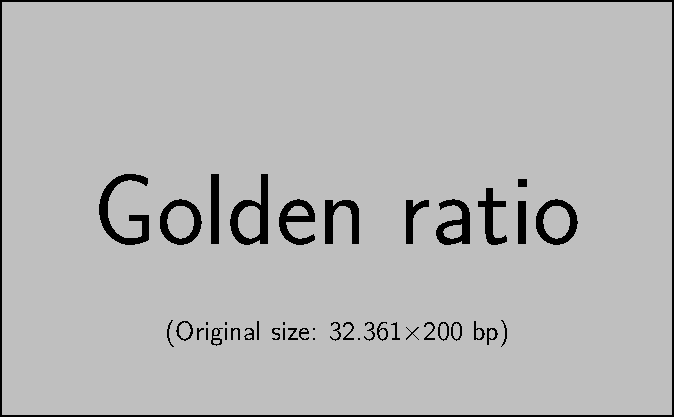
\includegraphics{placeholder_images/example-image-golden.pdf}
    \caption[Charge-transer and basic working mechanism of a Li-ion cell]{Simplified representation of charge-transfer
    process and illustration of basic working mechanism of a Li-ion cell.}
    \label{fig:chargetransferprocess}
\end{figure}

At fully  charged condition,  the majority  of Lithium in  the system  is stored
within the negative electrode  microstructure. During discharge, \ch{Li^0} atoms
diffuse out of  deep interstitial sites towards the surface  of the particles in
the  negative electrode.  At  the surface  (electrode-electrolyte interface),  a
charge-transfer process takes place according to Butler-Volmer kinetics, leading
to  the formation  of \ch{Li^+}  ions and  electrons. The  electrons are  passed
to  the external  circuit  through  \ch{Cu} current  collectors  onto which  the
conductive matrix  composed of  the negative electrode  material and  binders is
coated. The  \ch{Li^+} ions travel  through the electrolyte phase,  crossing the
separator membrane  to the positive  electrode where they encounter  an electron
influx from the external circuit. A  charge transfer reaction takes place at the
surface of the positive electrode particles, leading to the formation of neutral
\ch{Li^0} atoms that diffuse into the positive electrode microstructure.

During  the   charging  process,  the   reverse  phenomena  occur.   Lithium  is
de-intercalated  from  the  positive  electrode and  a  similar  charge-transfer
happens  at the  surface,  leading  to the  formation  of  \ch{Li^+} ions  which
reach  the  negative  electrode  by   passing  through  the  separator.  At  the
surface  of  the  negative  electrode particles,  these  ions  absorb  electrons
from  the  external circuit,  leading  to  the  formation of  neutral  \ch{Li^0}
that   diffuses  into   interior   vacant  spaces   in   the  layered   graphite
electrode. The  charge-transfer mechanism  and sequence  of events  are depicted
in~\cref{fig:chargetransferprocess}.
\Cref{eq:NegElectrodeRxn,eq:PosElectrodeRxn} summarise the reactions during the
charging and discharging process at the surfaces of both electrode materials.
\begin{align}
    \ch{Li_{$x$} C                            &<=>[\tiny{discharge}][\tiny{charge}] C + $x$ Li^+ + $x$ e^-}\label{eq:NegElectrodeRxn}\\
    \ch{Li_{1-$x$} M O2 + $x$ Li^+  + $x$ e^- &<=>[\tiny{discharge}][\tiny{charge}] LiMO2}\label{eq:PosElectrodeRxn}
\end{align}
where    \ch{M}   represents    a    transition   metal    compound   such    as
\ch{Ni_{1/3}Co_{1/3}Mn_{1/3}}   (NMC),   \ch{Ni_{0.8}Co_{0.15}Al_{0.05}}   (NCA)
amongst other  choices~\cite{Reddy2011}. Assuming  no loss of  cycleable Lithium
due to  parasitic side  reactions or  through other  mechanisms, the  process is
fully reversible.


The electrochemical potential at each electrode  is dependent upon the extent of
its  lithiation. An  empirical  relationship of  each  electrode's potential  as
a  function  of  its  stoichiometry  can be  obtained,  and  is  dependent  upon
the  specific design  and  material  properties of  each  active material  under
consideration. Finally, the \gls{ocv} of the cell is obtained by subtracting the
negative electrode potential from its positive electrode counterpart.

\subfile{1/dfn_equation_table}
